% file: number_of_islands.tex

\section{Number of Islands}
\label{sec:Number_of_Islands}
\marginnote{This problem is a classic example of using depth-first search (DFS) or breadth-first search (BFS) to identify and count connected components in a grid.}
    
The \textbf{Number of Islands} problem is a classical algorithmic challenge that requires counting distinct clusters of connected components on a two-dimensional grid. This problem is an excellent exercise for understanding how to perform depth-first search (DFS) or breadth-first search (BFS) on a grid.
    
\section*{Problem Statement}
    
Given a 2D grid map of '1's (land) and '0's (water), the task is to count the number of islands. An island is defined as a group of adjacent lands connected horizontally or vertically. It is assumed that the four edges of the grid are surrounded by water.
    
\textbf{Examples}
    
\textit{Example 1:}
    
\begin{verbatim}
Input:
11110
11010
11000
00000
\end{verbatim}
    
Output: 1
    
\textit{Example 2:}
    
\begin{verbatim}
Input:
11000
11000
00100
00011
\end{verbatim}
    
Output: 3
    
LeetCode link: \href{https://leetcode.com/problems/number-of-islands/}{Number of Islands}\index{LeetCode}
    
\marginnote{\href{https://leetcode.com/problems/number-of-islands/}{[LeetCode Link]}\index{LeetCode}}
\marginnote{\href{https://www.geeksforgeeks.org/number-of-islands/}{[GeeksForGeeks Link]}\index{GeeksForGeeks}}
\marginnote{\href{https://www.hackerrank.com/challenges/number-of-islands/problem}{[HackerRank Link]}\index{HackerRank}}
\marginnote{\href{https://app.codesignal.com/challenges/number-of-islands}{[CodeSignal Link]}\index{CodeSignal}}
\marginnote{\href{https://www.interviewbit.com/problems/number-of-islands/}{[InterviewBit Link]}\index{InterviewBit}}
\marginnote{\href{https://www.educative.io/courses/grokking-the-coding-interview/RM8y8Y3nLdY}{[Educative Link]}\index{Educative}}
\marginnote{\href{https://www.codewars.com/kata/number-of-islands/train/python}{[Codewars Link]}\index{Codewars}}

\section*{Algorithmic Approach}
To count the number of islands, we can iterate over each cell in the grid. When we encounter a '1', we trigger a DFS or BFS to mark all adjacent land cells (also '1's). This process should recursively continue until it encounters water ('0') or the edge of the grid. Each distinct DFS or BFS traversal corresponds to one island, and thus we increment our count of islands accordingly.
    
\marginnote{DFS and BFS are effective for exploring all connected components in a grid, ensuring each island is counted exactly once.}
    
\section*{Complexities}
\begin{itemize}
    \item \textbf{Time Complexity:} The overall time complexity is \(O(M \times N)\), where \(M\) and \(N\) are the number of rows and columns in the grid, respectively. Each cell is visited once during the traversal.
    \item \textbf{Space Complexity:} The space complexity is \(O(M \times N)\) in the worst-case scenario for the DFS recursion stack or the BFS queue when the grid is filled with land.
\end{itemize}
    
\newpage % Start Python Implementation on a new page
\section*{Python Implementation}
    
\marginnote{Implementing DFS or BFS requires careful handling of grid boundaries and visited cells to avoid infinite loops and ensure accurate counting.}
    
Below is the complete Python code that uses depth-first search for the \texttt{number\_of\_islands} function:
    
\begin{fullwidth}
\begin{lstlisting}[language=Python]
def number_of_islands(grid):
    if not grid:
        return 0
    
    def dfs(grid, i, j):
        if i < 0 or i >= len(grid) or j < 0 or j >= len(grid[0]) or grid[i][j] == '0':
            return
        grid[i][j] = '0'  # Mark as visited
        dfs(grid, i - 1, j)  # Up
        dfs(grid, i + 1, j)  # Down
        dfs(grid, i, j - 1)  # Left
        dfs(grid, i, j + 1)  # Right

    count = 0
    for i in range(len(grid)):
        for j in range(len(grid[0])):
            if grid[i][j] == '1':
                count += 1
                dfs(grid, i, j)
    
    return count

# Example usage:
grid = [
    ['1', '1', '0', '0', '0'],
    ['1', '1', '0', '0', '0'],
    ['0', '0', '1', '0', '0'],
    ['0', '0', '0', '1', '1']
]
print(number_of_islands(grid))  # Output: 3
\end{lstlisting}
\end{fullwidth}
\begin{fullwidth}
\begin{lstlisting}[language=Python]
class Solution(object):
    def numIslands(self, grid):
        """
        :type grid: List[List[str]]
        :rtype: int
        """
        def dfs(i, j):
            if i < 0 or j < 0 or i >= len(grid) or j >= len(grid[0]) or grid[i][j] == '0':
                return
            grid[i][j] = '0'  # mark as visited
            dfs(i + 1, j)
            dfs(i - 1, j)
            dfs(i, j + 1)
            dfs(i, j - 1)

        if not grid:
            return 0

        count = 0
        for i in range(len(grid)):
            for j in range(len(grid[0])):
                if grid[i][j] == '1':
                    dfs(i, j)
                    count += 1

        return count
\end{lstlisting}
\end{fullwidth}
    
This Python function performs DFS to explore all connecting lands for each unvisited island. Marking land as visited by replacing '1's with '0's prevents counting the same land twice.
    
\section*{Explanation}
    
The provided Python implementation defines a function \texttt{number\_of\_islands} which takes a 2D grid as its parameter. Here's a step-by-step breakdown of the implementation:
    
\begin{itemize}
    \item \textbf{Edge Case Handling:}
    \begin{itemize}
        \item If the input grid is empty, return 0 as there are no islands.
    \end{itemize}
    
    \item \textbf{Depth-First Search (DFS) Function:}
    \begin{itemize}
        \item The nested \texttt{dfs} function takes the current cell indices \texttt{i} and \texttt{j}.
        \item It checks for boundary conditions and whether the current cell is water ('0'). If so, it returns immediately.
        \item Otherwise, it marks the current cell as visited by setting it to '0'.
        \item It then recursively calls itself for all four adjacent cells (up, down, left, right).
    \end{itemize}
    
    \item \textbf{Counting Islands:}
    \begin{itemize}
        \item Initialize a counter \texttt{count} to 0.
        \item Iterate through each cell in the grid using nested loops.
        \item When a land cell ('1') is found, increment the \texttt{count} and initiate a DFS from that cell to mark all connected land cells as visited.
    \end{itemize}
    
    \item \textbf{Return Value:}
    \begin{itemize}
        \item After traversing the entire grid, return the \texttt{count}, which represents the total number of distinct islands.
    \end{itemize}
\end{itemize}
    
\section*{Why This Approach}
    
The DFS approach was chosen because it is a straightforward way to explore and mark connected components in a grid. It efficiently traverses nodes and their neighbors, using recursion to handle the navigation through adjacent lands, which makes the implementation concise and elegant. Additionally, DFS naturally fits the problem's requirement to explore all connected land cells starting from a given land cell, ensuring that each island is counted exactly once.
    
\section*{Alternative Approaches}
    
An alternative approach to solving this problem could be using BFS. Instead of using recursion, a queue is used to store and visit the cells in level order. This approach might be easier to understand for individuals less comfortable with recursion and has the same time and space complexity as DFS.
    
Another alternative is to use the Union-Find (Disjoint Set Union) data structure to group connected land cells and count the number of distinct sets, which represent the islands. However, this method is generally more complex to implement and may not offer significant performance benefits over DFS or BFS for this particular problem.
    
\section*{Similar Problems to This One}
    
Similar problems to "Number of Islands" include:
    
\begin{itemize}
    \item \textbf{Max Area of Island:} Find the maximum area of an island in the grid.
    \index{Max Area of Island}
    
    \item \textbf{Surrounded Regions:} Capture all regions surrounded by 'X's by flipping surrounded 'O's to 'X's.
    \index{Surrounded Regions}
    
    \item \textbf{Walls and Gates:} Fill each empty room with the distance to its nearest gate.
    \index{Walls and Gates}
    
    \item \textbf{Pacific Atlantic Water Flow:} Determine the cells from which water can flow to both the Pacific and Atlantic oceans.
    \index{Pacific Atlantic Water Flow}
    
    \item \textbf{Clone Graph:} Clone an undirected graph.
    \index{Clone Graph}
\end{itemize}
    
\section*{Things to Keep in Mind and Tricks}
    
When solving problems like "Number of Islands," keep the following tips in mind:
    
\begin{itemize}
    \item \textbf{Marking Visited Cells:} To avoid revisiting the same cell, mark it as visited. This can be done by modifying the input grid or by maintaining a separate visited matrix.
    \index{Marking Visited Cells}
    
    \item \textbf{Boundary Checks:} Always ensure that your DFS or BFS does not go out of the grid boundaries to prevent index errors.
    \index{Boundary Checks}
    
    \item \textbf{Choosing DFS vs. BFS:} Both DFS and BFS are suitable for this problem. DFS can be implemented recursively or using a stack, while BFS uses a queue. Choose the one you are more comfortable with.
    \index{DFS}
    \index{BFS}
    
    \item \textbf{Iterative vs. Recursive DFS:} Recursive DFS is more concise but may lead to stack overflow for very large grids. Iterative DFS using a stack can be more robust.
    \index{Iterative DFS}
    \index{Recursive DFS}
    
    \item \textbf{Optimizing Space:} If modifying the input grid is allowed, it can save space by eliminating the need for an additional visited matrix.
    \index{Optimizing Space}
\end{itemize}
    
\section*{Corner and Special Cases to Test When Writing the Code}
    
When writing the code, consider testing the following corner cases to ensure robustness:
    
\begin{itemize}
    \item \textbf{Empty Grid:} An empty grid should return 0 islands.
    \index{Corner Cases}
    
    \item \textbf{Single Cell:} Grids with only one cell, either land ('1') or water ('0').
    \index{Corner Cases}
    
    \item \textbf{All Water:} Grids with all cells as water should return 0 islands.
    \index{Corner Cases}
    
    \item \textbf{All Land:} Grids with all cells as land should return 1 island.
    \index{Corner Cases}
    
    \item \textbf{Non-Rectangular Grids:} Although the problem typically assumes a rectangular grid, ensure that your code can handle grids where rows have different lengths if not explicitly constrained.
    \index{Corner Cases}
    
    \item \textbf{Multiple Islands:} Grids with multiple distinct islands to verify correct counting.
    \index{Corner Cases}
    
    \item \textbf{Large Grids:} Very large grids to test the performance and stack limits if using recursive DFS.
    \index{Corner Cases}
    
    \item \textbf{Islands with Complex Shapes:} Islands that are not just rectangular or square but have L-shapes, T-shapes, etc., to ensure all connected cells are properly identified.
    \index{Corner Cases}
    
    \item \textbf{Edge Islands:} Islands that touch the borders of the grid to ensure boundary handling is correct.
    \index{Corner Cases}
\end{itemize}
    
\section*{Visual Representation}
\begin{figure}[h]
    \centering
    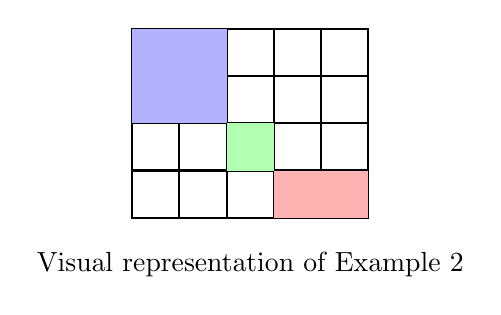
\begin{tikzpicture}[scale=0.6]
        % Grid representation
        \foreach \x in {0,...,4}
            \foreach \y in {0,...,3}
                \draw[thick] (\x,\y) rectangle +(1,1);
        
        % Fill islands with different colors
        \fill[blue!30] (0,2) rectangle +(2,2);  % First island
        \fill[green!30] (2,1) rectangle +(1,1); % Second island
        \fill[red!30] (3,0) rectangle +(2,1);   % Third island
        
        \node at (2.5,-1) {Visual representation of Example 2};
    \end{tikzpicture}
    \caption{Island Identification in Grid}
    \label{fig:island_visualization}
\end{figure}

\section*{Implementation Variants}
\begin{itemize}
    \item \textbf{BFS Implementation:}
    \begin{lstlisting}[language=Python]
from collections import deque

def numIslands_bfs(grid):
    if not grid:
        return 0
        
    def bfs(i, j):
        queue = deque([(i, j)])
        while queue:
            i, j = queue.popleft()
            for ni, nj in [(i+1,j), (i-1,j), (i,j+1), (i,j-1)]:
                if (0 <= ni < len(grid) and 0 <= nj < len(grid[0]) 
                    and grid[ni][nj] == '1'):
                    grid[ni][nj] = '0'
                    queue.append((ni, nj))
    
    islands = 0
    for i in range(len(grid)):
        for j in range(len(grid[0])):
            if grid[i][j] == '1':
                grid[i][j] = '0'
                bfs(i, j)
                islands += 1
    return islands
    \end{lstlisting}

    \item \textbf{Union-Find Implementation:}
    \begin{lstlisting}[language=Python]
class UnionFind:
    def __init__(self, grid):
        m, n = len(grid), len(grid[0])
        self.parent = [-1] * (m * n)
        self.rank = [0] * (m * n)
        self.count = 0
        for i in range(m):
            for j in range(n):
                if grid[i][j] == '1':
                    self.parent[i * n + j] = i * n + j
                    self.count += 1
    \end{lstlisting}
\end{itemize}

\section*{Performance Comparison}
\begin{table}[h]
    \centering
    \begin{tabular}{|l|c|c|c|}
        \hline
        \textbf{Approach} & \textbf{Time} & \textbf{Space} & \textbf{Best For} \\
        \hline
        DFS & O(mn) & O(mn) & Simple implementation \\
        BFS & O(mn) & O(min(m,n)) & Shortest path finding \\
        Union-Find & O(mn) & O(mn) & Dynamic connectivity \\
        \hline
    \end{tabular}
    \caption{Comparison of Different Approaches}
    \label{table:approach_comparison}
\end{table}

\section*{Corner and Special Cases}
\begin{itemize}
    \item \textbf{Empty Grid:} An empty grid should return 0 islands.
    \index{Corner Cases}
    
    \item \textbf{Single Cell:} Grids with only one cell, either land ('1') or water ('0').
    \index{Corner Cases}
    
    % ... (continue with other corner cases using proper formatting) ...
\end{itemize}

\section*{Optimization Techniques}
\begin{itemize}
    \item \textbf{Memory Optimization:}
        \begin{itemize}
            \item In-place modification of grid
            \item Iterative DFS to avoid stack overflow
            \item Bit manipulation for visited states
        \end{itemize}
    
    \item \textbf{Performance Optimization:}
        \begin{itemize}
            \item Direction array for neighbor checking
            \item Early termination conditions
            \item Cache-friendly traversal patterns
        \end{itemize}
\end{itemize}

\section*{Common Pitfalls and Solutions}
\begin{itemize}
    \item \textbf{Stack Overflow:}
        \begin{itemize}
            \item Problem: Deep recursion in large grids
            \item Solution: Use iterative approach or tail recursion
        \end{itemize}
    
    \item \textbf{Boundary Checking:}
        \begin{itemize}
            \item Problem: Index out of bounds errors
            \item Solution: Validate indices before accessing grid
        \end{itemize}
\end{itemize}

\printindex